\section{Habib Abdul Rasyid / 1174002}

\subsection{Teori}
\begin{enumerate}
\item Jelaskan apa itu klasifikasi teks, sertakan gambar ilustrasi buatan sendiri.\par
Klasifikasi teks yaitu cara untuk pemilihan teks yang mendasari parameter tertentu termasuk jenis teks atau dari kumpulan dokumen yang isinya penuh dengan teks, arti dari teks nya itu sendiri merupakan rangkaian kata yang dapat dibaca.

\begin{figure}[ht]
\centering
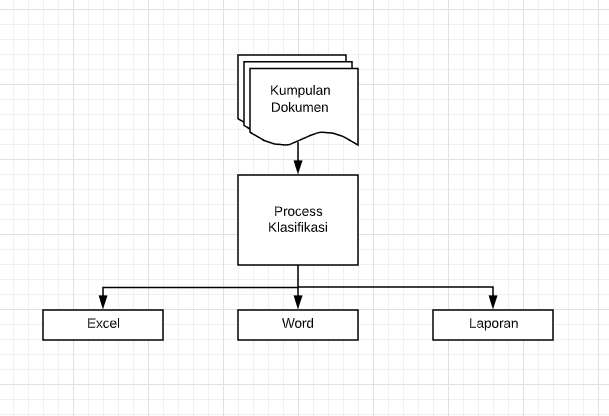
\includegraphics[scale=0.2]{figures/1174002/4/1.PNG}
\caption{contoh klasifikasi teks}
\label{contoh}
\end{figure}

\item Jelaskan mengapa klasifikasi bunga tidak bisa menggunakan machine learning, sertakan ilustrasi sendiri.\par
Klasisifikasi Bunga tidak dapat dimasukkan ke dalam mesin learning karena jenis-jenis bunga kebanyakan hampir mirip atau memiliki ciri ciri yang sama namun tidak mirip. Hal itu yang menyebabkan klasifikasi bunga tidak bisa digunakan oleh mesin learning.

\begin{figure}[ht]
\centering
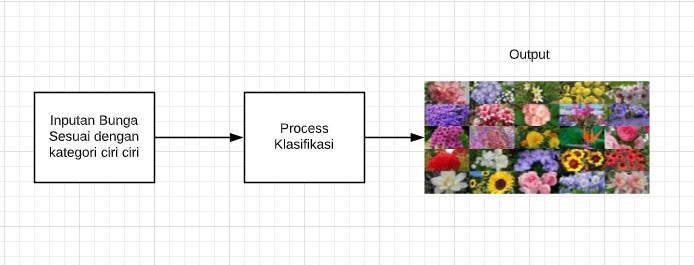
\includegraphics[scale=0.2]{figures/1174002/4/2.PNG}
\caption{contoh klasifikasi bunga}
\label{contoh}
\end{figure}

\item Jelaskan bagaimana teknik pembelajaran mesin pada teks pada kata-kata yang digunakan di youtube,jelaskan arti per atribut data csv dan sertakan ilustrasi buatan sendiri.\par
Cara Pembelajaran teks yang ada pada youtube yaitu dengan cara merekam jejak penelusuran yang sering dicari dan terakhir kali dicari sebelumnya, kita bisa melihat ini pada menu pencarian youtube dan history youtube. namun pada contoh dibawah ini menggunakan menu pencarian youtube untuk melihat teks yang terakhir kali dicari di youtube hanya dengan klik pada kolom pencarian.

\begin{figure}[ht]
\centering
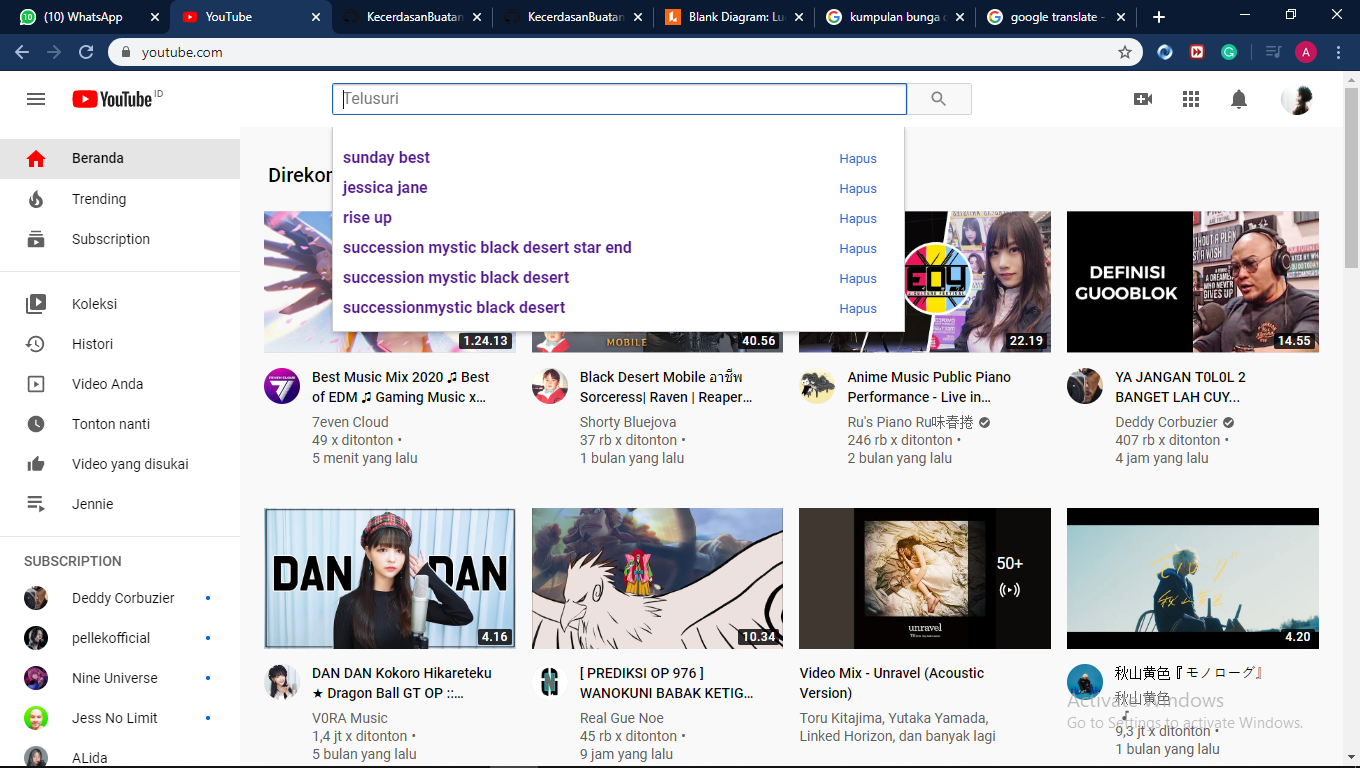
\includegraphics[scale=0.2]{figures/1174002/4/3.PNG}
\caption{contoh teknik pembelajaran mesin}
\label{contoh}
\end{figure}

\item Jelaskan apa yang dimaksud vektorisasi data.\par
vektorisasi data merupakan pemechan data menjadi bagian bagian yang lebih sederhana contoh pada satu paragraf terdiri dari 200 kata kemudian dilakukan vektorisasi dengancara membagi-bagi kata dalam paragraf tersebut ke dalam kalimat-kalimat yang terpisah kemudian di pecah lagi menjadi data dalam perkata selanjutnya kata kata tersebut di terjemahkan.

\item Jelaskan apa itu bag of words dengan kata-kata yang sederhana dan ilustrasi sendiri.\par
 bag of words merupakan peroses penyederhanaan kata-kata, Misalnya Satu kalimat diubah menjadi perkata dan dikelompokkan lalu akan dilakukan perhitungan frekuensi kemunculan setiap kata katanya.
\begin{figure}[ht]
\centering
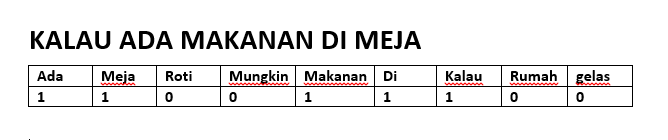
\includegraphics[scale=0.2]{figures/1174002/4/4.PNG}
\caption{contoh bag of words}
\label{contoh}
\end{figure}

\item Jelaskan apa itu TF-IDF, ilustrasikan dengan gambar sendiri.
 TF-IDF merupakan metode untuk menghitung bobot dari kata yang sering muncul pada suatu kalimat. metode ini menghitung nilai TF atau Term Frequency dan IDF atau Inverse Document Frequency pada setiap kata pada kalimat yang dijadikan acuan kata pada metode ini sering di sebut token.
 
\begin{figure}[ht]
\centering
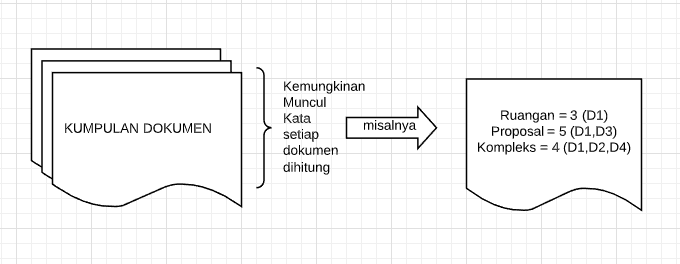
\includegraphics[scale=0.2]{figures/1174002/4/5.PNG}
\caption{contoh TF-IDF}
\label{contoh}
\end{figure}

\end{enumerate}

\subsection{Praktek Program}
\begin{enumerate}
\item import data pandas dan 500 baris data dumy kemudian di jelaskan tiap barisnya.
\lstinputlisting{src/1174002/chapter4/2,1.py}


\item memecah data prame menjadi dua yag pertama 450 dan kedua sisanya
\lstinputlisting{src/1174002/chapter4/2,2.py}

\item praktek vektorisasi\par
berikut merupakan codingan untuk melakukan vektorisasii data berupa teks dalam vormat csv
\lstinputlisting{src/1174002/chapter4/2,3.py}
\begin{figure}[ht]
\centering
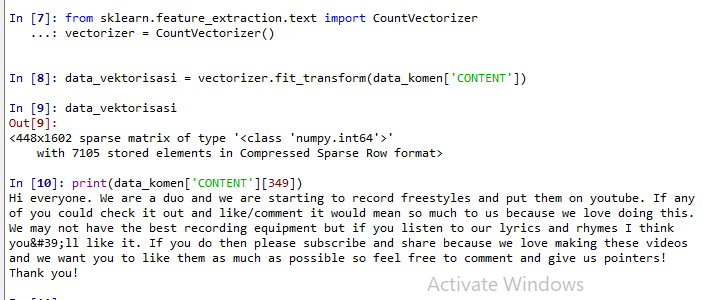
\includegraphics[scale=0.5]{figures/1174002/4/ss1.PNG}
\caption{hasil}
\label{Praktek no 3}
\end{figure}
lakukan import library pandas yang di inisialisasi menjasi pd setelah itu ada dibuat class data\_komen dengan method read\_csv untuk membaca file berekstensikan csv yang di masukan alamatnya pada kurung, lakukan klasifikasi atau pemilihan komentar yang berisi spam atau bukan spam dengan parameter class samadengan 1 merupakan spam dan class samadengan 0 bukan spam setelah itu masukan librari CountVektorizer yang digunakan untuk vektorisasi data kemudian dilanjutkan pada bagian In[103] dibuat variabel yang berisi vektorisasi dari data pada data\_komen di field content setelah itu variabel tersebut di running hasilnya menunjukan 350 baris di kali 1738 kolom selanjutnya dicoba untuk memunculkan isi recod pada baris ke 349 maka akan muncul isian dari baris tersebut. 

\item klasifikasi SVM
berikut ini merupakan codingan klasifikasi SVM 
\lstinputlisting{src/1174002/chapter4/2,4.py}
\begin{figure}[ht]
\centering
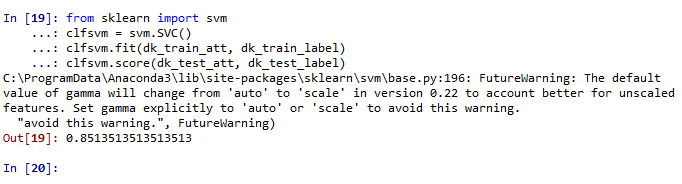
\includegraphics[scale=0.5]{figures/1174002/4/ss2.PNG}
\caption{hasil}
\label{Praktek no 4}
\end{figure}
melakukan verifikasi import librari svm dari sklearn kemudian membuat variabel clfsvm berisikan method svc setelah itu variabel tersebut di berikan method fit dengan isian data train vektorisasi dan data training label yang berguna untuk melatih data tersebut setelah itu di coba untuk memunculkan score atau akurasi dari data tersebut menggunakan data testing vektorisasi dan data testing label.

\item klasifikasi decision tree 
berikut ini merupakan codingan klasifikasi decision tree
\lstinputlisting{src/1174002/chapter4/2,5.py}
\begin{figure}[ht]
\centering
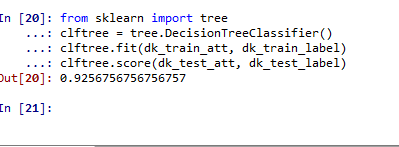
\includegraphics[scale=0.5]{figures/1174002/4/ss3.PNG}
\caption{hasil}
\label{Praktek no 5}
\end{figure}
melakukan verifikasi import librari tree dari sklearn kemudian membuat variabel clftree berisikan method DecisionTreeClasifier setelah itu variabel tersebut di berikan method fit dengan isian data train vektorisasi dan data training label yang berguna untuk melatih data tersebut agar dapat digunakan pada codingan selanjutnya setelah itu di coba untuk memunculkan score atau akurasi dari data tersebut menggunakan data testing vektorisasi dan data testing label.

\item plot comfusion matrix
berikut merupakan codingan untuk confusion matrix 
\lstinputlisting{src/1174002/chapter4/2,6.py}

lakukan import library comfusion matrix selanjutnya dilakukan prediksi pada pada data tes nya kemudian data tersebut di masukan kedalam variabel cm dengan method confusion matrix yang di dalamnya terdapat data dari variabel perd label dan dk test label setelah itu variabel cm tersebut di running maka akan memunculkan nilai matrixnya. 

\item cross valodation 
berikut merupakan code untuk cross validation pada codingan pertama yaitu melakukan split 5 kali yaoti mengitung tingkat akurasi menggunakan data training.
\lstinputlisting{src/1174002/chapter4/2,7.py}

memunculkan nilai akurasi dari tiga metode yaitu random forest, decision tree, dan klasifikasi svm (suport vector machine) diamana akan di bandingkan tingkat akurasi dari semua hasil akurasiya mana yang terbaik dan lebih akurat pada hasilnya data yang paling akurat yaitu random forest.



\end{enumerate}
\subsection{Penanganan Error}
\begin{enumerate}
\item screnn shoot error

\begin{figure}[ht]
\centering
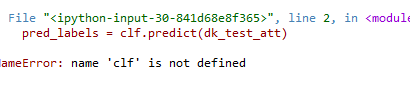
\includegraphics[scale=0.5]{figures/1174002/4/ss4.PNG}
\caption{hasil}
\label{Error}
\end{figure}

\item codingan yang errornya terdapat pada 
\begin{verbatim}
clfsvm.fit(dk_train_att, d_train_label)
\end{verbatim}
\item solusinya
\begin{verbatim}
clfsvm.fit(dk_train_att, dk_train_label)
\end{verbatim}
\end{enumerate}
